\documentclass{article}

\usepackage{graphicx}
\usepackage{tikz}
\usepackage{tikzsymbols}
\usetikzlibrary{calc,patterns,shapes.geometric}
\pagestyle{empty}
\usepackage[margin=0pt]{geometry}
\geometry{papersize={14in,12in}}

\def\centerarc[#1](#2)(#3:#4:#5){\draw[#1] ($(#2)+({#5*cos(#3)},{#5*sin(#3)})$) arc (#3:#4:#5);}

\begin{document}
	\begin{figure}
		\centering
		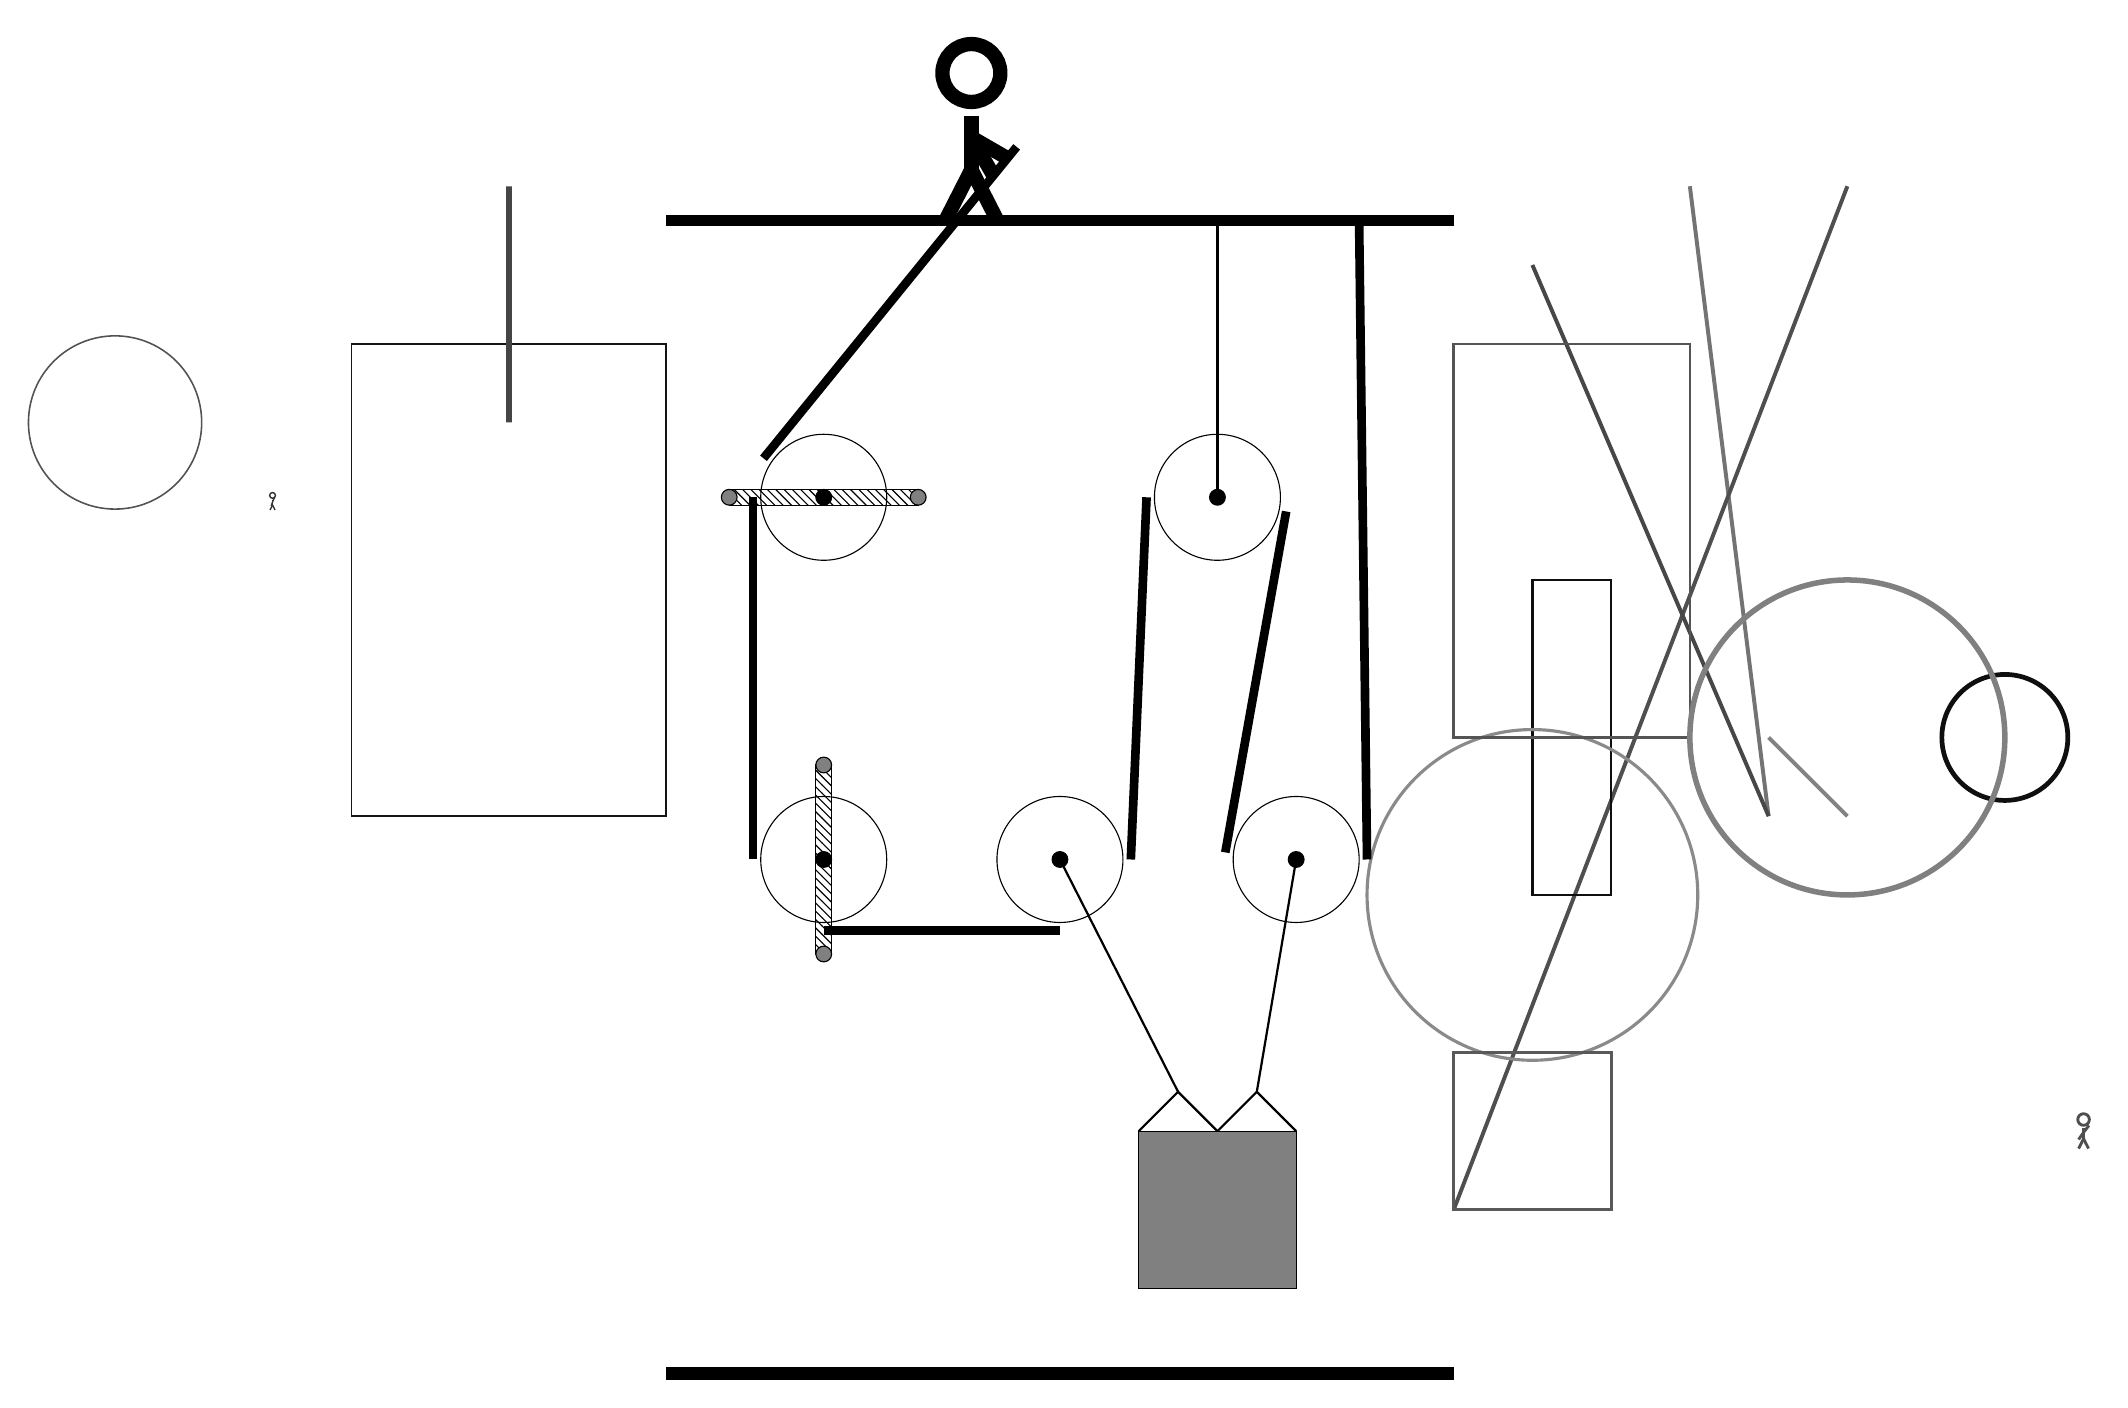
\begin{tikzpicture}
			%%%%% START %%%%%
			
			\draw[fill=black] (-4, 11.5) rectangle (6, 11.625);
			
			\draw (1, 3.45) circle (0.8);
			\draw[fill=black] (1, 3.45) circle (0.1);
			
			\draw (3, 8.05) circle (0.8);
			\draw[fill=black] (3, 8.05) circle (0.1);
			\draw[thick] (3, 8.05) -- (3, 11.5);
			
			\draw (4, 3.45) circle (0.8);
			\draw[fill=black] (4, 3.45) circle (0.1);
			
			\draw[thick] (4, 3.45) -- (3.5, 0.5);
			\draw[thick] (1, 3.45) -- (2.5, 0.5);
			\draw[thick]  (2, 0) -- (2.5, 0.5) -- (3, 0);
			\draw[thick]  (3, 0) -- (3.5, 0.5) -- (4, 0);
			\draw[fill=black!50] (2, 0) rectangle (4, -2);
			
			\draw[line width=0.5mm, color=black!55](10, 4) -- (9, 12);
			
			\draw[line width=0.2mm, color=black!92] (-4, 10) rectangle (-8, 4);
			\draw[line width=0.5mm, color=black!69](11, 12) -- (6, -1);
			\draw[line width=0.7mm, color=black!73] (-6, 9) rectangle (-6, 12);
			\draw[line width=0.4mm, color=black!68] (7, 5) rectangle (8, 5);
			
			\node[line width=0.3mm, color=black!80] at (-9, 8) {\Strichmaxerl[1][73][66]};
			
			\draw[line width=0.3mm, color=black!94] (7, 3) rectangle (8, 7);
			\draw [line width=0.2mm, color=black!68](-11, 9) circle (1.1);
			\draw [line width=0.4mm, color=black!46](7, 3) circle (2.1);
			
			\draw[line width=0.5mm, color=black!72](7, 11) -- (10, 4);
			
			\node[line width=0.6mm, color=black!69] at (14, 0) {\Strichmaxerl[2][55][52]};
			\draw[line width=0.3mm, color=black!67] (6, 10) rectangle (9, 5);
			\draw[line width=0.4mm, color=black!65] (8, 1) rectangle (6, -1);
			
			\draw [line width=0.6mm, color=black!94](13, 5) circle (0.8);
			\draw [line width=0.7mm, color=black!50](11, 5) circle (2.0);
			\draw[line width=0.5mm, color=black!49](11, 4) -- (10, 5);
			
			
			\draw (-2, 3.45) circle (0.8);
			\draw[fill=black] (-2, 3.45) circle (0.1);
			\draw[pattern=north west lines, pattern color=black] (-2.1, 4.65) rectangle (-1.9, 2.25);
			\draw[fill=black!50] (-2, 4.65) circle (0.1);
			\draw[fill=black!50] (-2, 2.25) circle (0.1);
			
			\draw (-2, 8.05) circle (0.8);
			\draw[fill=black] (-2, 8.05) circle (0.1);
			\draw[pattern=north west lines, pattern color=black] (-3.2, 8.15) rectangle (-0.8, 7.95);
			\draw[fill=black!50] (-3.2, 8.05) circle (0.1);
			\draw[fill=black!50] (-0.8, 8.05) circle (0.1);
			
			\draw[line width=1.1mm] (0.45, 12.5) -- (-2.765, 8.545);
			\centerarc[line width=1.1mm](-2, 8.05)(135:180:0.9);
			\draw[line width=1.1mm] (-2.9, 8.05) -- (-2.9, 3.45);
			\centerarc[line width=1.1mm](-2, 3.45)(180:270:0.9);
			\draw[line width=1.1mm](-2, 2.55) -- (1, 2.55);
			\centerarc[line width=1.1mm](1, 3.45)(270:360:0.9);
			\draw[line width=1.1mm] (1.9, 3.45) -- (2.1, 8.05);
			\centerarc[line width=1.1mm](3, 8.05)(-20:180:0.9);
			\draw[line width=1.1mm](3.873, 7.87) -- (3.1, 3.54);
			\centerarc[line width=1.1mm](4, 3.45)(160:360:0.9);
			\draw[line width=1.1mm](4.9, 3.45) -- (4.8, 11.5);
			
			\node at (-0.07, 12.7) {\Strichmaxerl[10][120][-30]};
			
			\draw[fill=black] (-4, -3) rectangle (6, -3.15);
			
			%%%%% END %%%%%
		\end{tikzpicture}
	\end{figure}	
\end{document}